\chapter{Autonomous Navigation Method}
\label{mainone}
\textit{
DELETEME: In this chapter you start addressing your actual problem. Therefore, it makes often sense to make a detailed problem analysis first (if not done in introduction). You should be sure about what to do and how. As writtin in the background part, it might also make sense to include complex background information or papers you are basing on in this analysis. If you are solving a software problem, you should follow the state of the art of software development which basically includes: problem analysis, design, implementation, testing, and deployment. Maintenance is often also described but I believe this will not be required for most theses. Code should be placed in the appendix unless it is solving an essential aspect of your work.
}





In order to investigate the effect of temporal comprehension in machine-learning-based, autonomous navigation of drones,
this master thesis extends the navigation method of Kaufmann, Loquercio et. al [?] is minimally adjusted and extended with a recurrent convolutional neural network.
This chapter \dots



\section{Reference systems}
In this thesis, the coordinates of a point 
$\pos[]{}{}{}{}$
relate to either the global, the local or the image reference system
\begin{equation}
    \pos[]{}{}{\grs}{} = \begin{bmatrix}
        \x[]{}{}{\grs}{} \\ \y[]{}{}{\grs}{} \\ \z[]{}{}{\grs}{}
    \end{bmatrix} \in \mathbb{R}^3
    ,\quad 
    \pos[]{}{}{\lrs}{} = \begin{bmatrix}
        \x[]{}{}{\lrs}{} \\ \y[]{}{}{\lrs}{} \\ \z[]{}{}{\lrs}{}
    \end{bmatrix} \in \mathbb{R}^3
    ,\quad 
    \pos[]{}{}{\irs}{} = \begin{bmatrix}
        \x[]{}{}{\irs}{} \\ \y[]{}{}{\irs}{}
    \end{bmatrix} \in \left[\text -1, 1\right]^2.
\end{equation}


The 3D global reference system
is fixed to an arbitrary point on earth
and is hence quasi inertial.
It is spanned by the orthonormal basis
which, related to the global reference system,
equates to the standard basis of $\mathbb{R}^3$
\begin{equation}
    \left\{
        \unitvec[]{\text G}{x}{}{},
        \unitvec[]{\text G}{y}{}{},
        \unitvec[]{\text G}{z}{}{}
    \right\}
    \quad \text{with} \quad 
    \unitvec[]{\text G}{x}{\grs}{} = \begin{bmatrix} 1 \\ 0 \\ 0 \end{bmatrix},\ 
    \unitvec[]{\text G}{y}{\grs}{} = \begin{bmatrix} 0 \\ 1 \\ 0 \end{bmatrix},\ 
    \unitvec[]{\text G}{z}{\grs}{} = \begin{bmatrix} 0 \\ 0 \\ 1 \end{bmatrix}.
\end{equation}


The local reference system (see figure \ref{fig:local_reference_system}) is fixed to the moving drone.
It is spanned by the orthonormal basis,
whose origin is located at the optical center of the drone's onboard camera,
\begin{equation}
    \left\{
        \unitvec[]{\text L}{x}{}{},
        \unitvec[]{\text L}{y}{}{},
        \unitvec[]{\text L}{z}{}{}
    \right\}
    \quad \text{with} \quad 
    \unitvec[]{\text L}{x}{\lrs}{} = \begin{bmatrix} 1 \\ 0 \\ 0 \end{bmatrix},\ 
    \unitvec[]{\text L}{y}{\lrs}{} = \begin{bmatrix} 0 \\ 1 \\ 0 \end{bmatrix},\ 
    \unitvec[]{\text L}{z}{\lrs}{} = \begin{bmatrix} 0 \\ 0 \\ 1 \end{bmatrix}.
\end{equation}
The unit vector 
$\unitvec[]{\text L}{x}{}{}$ 
points along the optical axis of the camera
in the flight direction of the drone.
The unit vector
$\unitvec[]{\text L}{z}{}{}$ 
points in the direction of the forces generated by the drone's rotors
and is parallel to the vertical axis of the image plane of the drone's onboard camera.
The unit vector 
$\unitvec[]{\text L}{y}{}{}$ 
points to the left of the drone
and parallels the horizontal axis of the image plane.






The image reference system (see figure \ref{fig:image_reference_system}) 
is superimposed on the images of the drone's onboard camera.
This 2-dimensional system is spanned by the orthonormal basis
\begin{equation}
    \left\{
        \unitvec[]{\text I}{x}{}{},
        \unitvec[]{\text I}{y}{}{}
    \right\}
    \quad \text{with} \quad 
    \unitvec[]{\text I}{x}{\irs}{} = \begin{bmatrix} 1 \\ 0 \end{bmatrix},\ 
    \unitvec[]{\text I}{y}{\irs}{} = \begin{bmatrix} 0 \\ 1 \end{bmatrix}.
\end{equation}
The origin of the image reference system 
is located at the center of the image plane.
The unit vector 
$\unitvec[]{\text I}{x}{}{}$  
points rightwards along the vertical axis of the image plane.
The unit vector 
$\unitvec[]{\text I}{y}{}{}$  
points upwards along the horizontal axis of the image plane.
A point on the image plane 
is bounded by the left and right
$ -1 \le \x[]{}{}{\irs}{} \le 1 $
as well as the lower and upper
$ -1 \le \y[]{}{}{\irs}{} \le 1 $
border of the image plane.
%The global reference system 
%is only referred to 
%by the expert system (see section)
%which makes navigation decisions based on globally consistent information
%when generating training data for the ANN module.
%The autonomous navigation method, 
%with the fully trained ANN module making the navigation decisions,
%exclusively resorts to data from onboard sensors,
%which is relative to the drone and its onboard camera.
%The method, therefore, operates only within the local and image reference system.
\begin{figure}[h]
    \centering
    \subfloat[
        Local reference system
    ]{
        \label{fig:local_reference_system}
        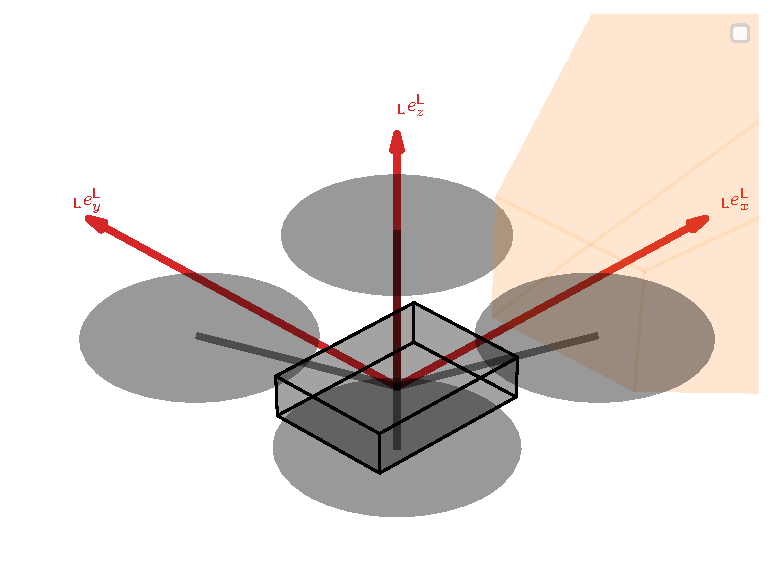
\includegraphics[width=0.441\textwidth]{own/local_reference_system.pdf}
    }                
    \subfloat[
        Image reference system
    ]{
        \label{fig:image_reference_system}
        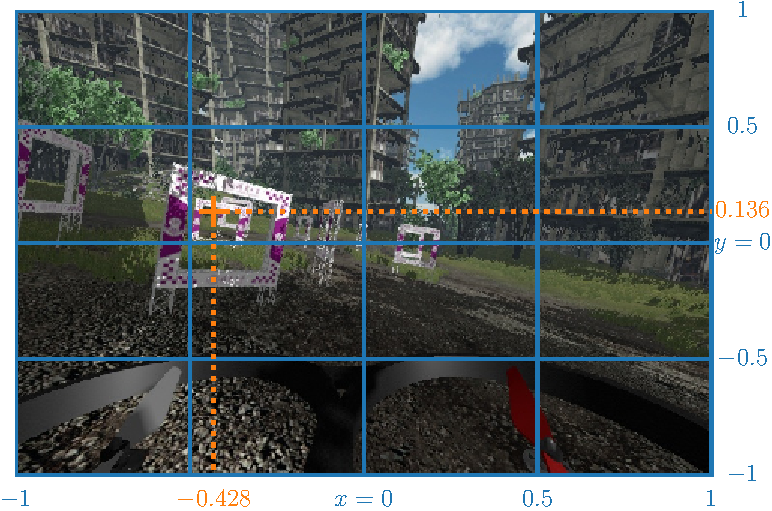
\includegraphics[width=0.5\textwidth]{own/image_reference_system.pdf}
    }
    \caption[
        The local and the image reference system
    ]{
        The local and the image reference system. 
        The local reference system (red) is aligned with the drone's onboard camera. 
        The image reference system (blue) is superimposed on the images from the onboard camera.
        The pictured, exemplary waypoint
        $\pos[]{\wayp}{}{\irs}{} = \begin{bmatrix} -0.428 & 0.136 \end{bmatrix}^T$
        (orange) with respect to the image reference system
        is part of the label for the underlying image.
        \label{fig:local_and_image_reference_system}
    }
\end{figure}
%https://www.researchgate.net/figure/Pin-hole-camera-model-terminology-The-optical-center-pinhole-is-placed-at-the-origin_fig10_317498100





\paragraph*{Transformation between the global and the local reference system} $\ $\\
The drone's position
$\pos[]{\drone}{}{\grs}{}$
and quaternion orientation
$\quat[]{\drone}{}{\grs}{}$
with respect to the global reference system
are the parameters that determine the bidirectional transformation
between the global and the local reference system.
The following bases on quaternion mathematics,
for which one can consult, e.g., \cite{Parent}.
A point given in the coordinates of the global reference system
can be expressed in the coordinates of the local reference system
with the transformation
\begin{align} \label{equ:global_to_local_transformation}
    \trafo[]{}{\lrs\grs}{}{}
    :\ 
    \mathbb{R}^3 \rightarrow \mathbb{R}^3
    ; \quad
    \pos[]{}{}{\grs}{} \mapsto \pos[]{}{}{\lrs}{}
    =
    %\begin{cases}
        \mathcal{P} \left[
            \mathrm{inv} \left( \quat[]{\drone}{}{\grs}{} \right)
            *
            \mathcal{Q} \left( \pos[]{}{}{\grs}{} - \pos[]{\drone}{}{\grs}{} \right)
            *
            \quat[]{\drone}{}{\grs}{}
        \right], 
        %& \text{if } \quat[]{\drone}{}{\grs}{} \ne \underline 0 \\
        %\pos[]{}{}{\grs}{} - \pos[]{\drone}{}{\grs}{}, 
        %& \text{else}.
    %\end{cases}
\end{align}
Reversely, a point given in the coordinates of the local reference system
can be expressed in the coordinates of the global reference system
with the transformation
\begin{align} \label{eq:local_to_global_transformation}
    \trafo[]{}{\grs\lrs}{}{}
    :\ 
    \mathbb{R}^3 \rightarrow \mathbb{R}^3
    ; \quad
    \pos[]{}{}{\lrs}{} \mapsto \pos[]{}{}{\grs}{}
    =
    %\begin{cases}
        \mathcal{P} \left[
            \quat[]{\drone}{}{\grs}{}
            *
            \mathcal{Q} \left( \pos[]{}{}{\lrs}{} \right)
            *
            \mathrm{inv} \left( \quat[]{\drone}{}{\grs}{} \right)
        \right] + \pos[]{\drone}{}{\grs}{}, 
        %& \text{if } \quat[]{\drone}{}{\grs}{} \ne \underline 0 \\
        %\pos[]{}{}{\lrs}{} + \pos[]{\drone}{}{\grs}{}, 
        %& \text{else}.
    %\end{cases}
\end{align}
In the two above transformations,
the mapping $\mathcal{Q}$
of a point to its quaternion representation 
and the reverse mapping $\mathcal{P}$ 
of a quaternion representation to its point  
are given by
\begin{align}
    \mathcal{Q}
    :\ 
    & \mathbb{R}^3 \rightarrow \mathbb{R}^4
    ;\
    \pos[]{}{}{}{} = \begin{bmatrix} \x[]{}{}{}{} \\ \y[]{}{}{}{} \\ \z[]{}{}{}{} \end{bmatrix} 
    \mapsto
    \quat[]{}{}{}{} = \begin{bmatrix} w \\ \underline p \end{bmatrix} 
    \text{ with } w = 0
    \nonumber \\
    \mathcal{P}
    :\ 
    &\mathbb{R}^4 \rightarrow \mathbb{R}^3
    ;\
    \quat[]{}{}{}{} = \begin{bmatrix} w \\ \underline p \end{bmatrix} 
    \mapsto
    \pos[]{}{}{}{} = \begin{bmatrix} \x[]{}{}{}{} \\ \y[]{}{}{}{} \\ \z[]{}{}{}{} \end{bmatrix}.
\end{align}
Moreover, the operator $*$ denotes the multiplication of two quaternions which is given by
\begin{align}
    \quat[]{}{1}{}{} * \quat[]{}{2}{}{}
    = 
    \begin{bmatrix}
        w_1 w_2 - \pos[]{T}{1}{}{} \pos[]{}{2}{}{}\\ 
        w_1 \pos[]{}{2}{}{} + w_2 \pos[]{}{1}{}{} + \pos[]{}{1}{}{} \times \pos[]{}{2}{}{}
    \end{bmatrix}.
\end{align}
Finally, the inversion of a quaternion is given by
\begin{align}
    \mathrm{inv}(\quat[]{}{}{}{}) 
    = 
    \frac{1}{\| \quat[]{}{}{}{} \|_2}
    \begin{bmatrix} w \\ \text - \pos[]{}{}{}{} \end{bmatrix}.
\end{align}
The two above transformations are the inversion of each other.
Therefore, points can be transformed between the global and local reference system
without information loss
\begin{equation}
    \trafo[]{}{\grs\lrs}{}{} \circ \trafo[]{}{\lrs\grs}{}{} 
    \left( \pos[]{}{}{\grs}{} \right)
    =
    \pos[]{}{}{\grs}{}
    ,\quad
    \trafo[]{}{\lrs\grs}{}{} \circ \trafo[]{}{\grs\lrs}{}{} 
    \left( \pos[]{}{}{\lrs}{} \right)
    =
    \pos[]{}{}{\lrs}{}.
\end{equation}
In the above equations, the operator $\circ$ denotes the composition of two functions.



\paragraph*{Transformation between the local and the image reference system} $\ $\\
The horizontal
$\ang[\user]{\camera}{\text h}{}{}$
and the vertical
$\ang[\user]{\camera}{\text v}{}{}$
angle of view
of the drone's onboard camera
are the parameters 
that determine the bidirectional transformation 
between the local and the image reference system.
A point given in the coordinates of the local reference system
is expressed in the coordinates of the image reference system with the transformation
\begin{align} \label{equ:local_to_image_transformation}
    \trafo[]{}{\irs\lrs}{}{}
    :\ 
    \mathbb{R}^3 \rightarrow \left[ \text{-}1, 1 \right]^2
    ; \quad
    \pos[]{}{}{\lrs}{} \mapsto \pos[]{}{}{\irs}{}
    =
    \begin{bmatrix}
        \maxof{\text -1}{
            \minof{
                \frac{\text -2}{\ang[\user]{\camera}{\text h}{}{}}
                \mathrm{atan2}\left( \y[]{}{}{\lrs}{}, \x[]{}{}{\lrs}{} \right)
            }{1}
        }
        \\
        \maxof{\text -1}{
            \minof{
                \frac{2}{\ang[\user]{\camera}{\text v}{}{}}
            \mathrm{atan2} \left( \z[]{}{}{\lrs}{}, \| \pos[]{}{}{\lrs}{} \|_2 \right)
            }{1}
        }
    \end{bmatrix}
    .
\end{align}
The above transformation
can be interpreted as the projection of a point onto the image plane 
of the drone's onboard camera.
It can be devided into three steps.
First, the vector from the optical center of the camera 
to the point to be transformed
is mapped to its yaw
$\mathrm{atan2}\left( \y[]{}{}{\lrs}{}, \x[]{}{}{\lrs}{} \right)$
and pitch 
$\mathrm{atan2} \left( \z[]{}{}{\lrs}{}, \| \pos[]{}{}{\lrs}{} \|_2 \right)$
angle, both, with respect to the image reference system.
Second these angles are normalized by 
the half of the horizontal 
$\ang[\user]{\camera}{\text h}{}{}$ 
and the half of the vertical
$\ang[\user]{\camera}{\text v}{}{}$
angle of view of the camera, respectively.
Third, these normalized angles are bounded to be in the interval from minus to plus one.
This boundary takes into account 
that an artifical neural network, which inputs images, 
has no basis for predictions 
that relate to objects that are not within the camera's field of view.
As a projection from 3D to 2D, the above transformation is accompanied by information loss
and is hence not bijective.

A point given in the coordinates of the image reference system is expressed
in the coordinates of the local reference system with the reverse transformation
\begin{align} \label{eq:image_to_local_transformation}
    \trafo[]{}{\lrs\irs}{}{}
    &:\ 
    \mathbb{R}_{\ge 0}, \left[ \text{-}1, 1 \right]^2 \rightarrow \mathbb{R}^3
    ; \quad
    d, \pos[]{}{}{\irs}{} \mapsto \pos[]{}{}{\lrs}{}
    =
    d \begin{bmatrix}
        \cos \left( \ang[]{}{y}{\lrs}{} \right) \\
        \cos \left( \ang[]{}{y}{\lrs}{} \right) \\
        \sin \left( \ang[]{}{y}{\lrs}{} \right)
    \end{bmatrix} \odot \begin{bmatrix}
        \cos \left( \ang[]{}{z}{\lrs}{} \right) \\
        \sin \left( \ang[]{}{z}{\lrs}{} \right) \\
        1
    \end{bmatrix}
    \nonumber \\
    & \qquad \text{with} \quad
    \ang[]{}{z}{\lrs}{}
    = 
    \text - \frac{\ang[\user]{\camera}{\text h}{}{}}{2} \cdot \x[]{}{}{\irs}{}
    ,\quad 
    \ang[]{}{y}{\lrs}{}
    = 
    \frac{\ang[\user]{\camera}{\text v}{}{}}{2} \cdot \y[]{}{}{\irs}{}.
\end{align}
In the above transformation,
the operator 
$\odot$ 
denotes the Hadamard product, 
i.e., the element-wise product of two equally dimensioned matrices.
Because the 2D coordinates of the image reference system
can only contain information about the direction of a point,
the above transformation to 3D requires the additional input of a backprojection length $d$.

In contrast to the transformations 
$\trafo[]{}{\lrs\grs}{}{}$
and 
$\trafo[]{}{\grs\lrs}{}{}$
between the global and the local reference system,
the transformations 
$\trafo[]{}{\irs\lrs}{}{}$
and 
$\trafo[]{}{\lrs\irs}{}{}$
between the local and the image reference system
are not invertible.
However, for relevant points
located within the camera's field of view
and a well chosen backprojection length,
it is assumed that the transformations approximately invert each other
\begin{equation}
    \trafo[]{}{\lrs\irs}{}{} \left[
        d, \trafo[]{}{\irs\lrs}{}{} \left( \pos[]{}{}{\lrs}{} \right)
    \right]
    \approx
    \pos[]{}{}{\lrs}{}
    ,\quad
    \trafo[]{}{\irs\lrs}{}{}
    \circ 
    \trafo[]{}{\lrs\irs}{}{} \left(
        d, \pos[]{}{}{\irs}{}
    \right)
    \approx
    \pos[]{}{}{\irs}{}.
\end{equation}





\paragraph*{Transformation between the global and the image reference system} $\ $\\
The bidirectional transformations of points between the global and the image reference frame
are the compositions of the transformations via the intermittent local reference system
\begin{align} \label{eq:global_image_transformations}
    \trafo[]{}{\irs\grs}{}{}
    &=
    \trafo[]{}{\irs\lrs}{}{} \circ \trafo[]{}{\lrs\grs}{}{}
    :\ 
    \mathbb{R}^3 \rightarrow \left[\text{-} 1, 1\right]^2 
    \nonumber \\
    \trafo[]{}{\grs\irs}{}{}
    &=
    \trafo[]{}{\grs\lrs}{}{} \circ \trafo[]{}{\lrs\irs}{}{}
    :\ 
    \mathbb{R}_{\ge 0}, \left[\text{-} 1, 1\right]^2 \rightarrow \mathbb{R}^3.
\end{align}
Due to the fact that
$\trafo[]{}{\lrs\grs}{}{}$
and
$\trafo[]{}{\grs\lrs}{}{}$
are the inverse of each other
and the assumption that
$\trafo[]{}{\irs\lrs}{}{}$
and
$\trafo[]{}{\lrs\irs}{}{}$
approximately invert each other within a relevant range,
the above compositions are expected to also approximately invert each other within this relevant range
\begin{equation}
    \trafo[]{}{\grs\irs}{}{} \left[
        d, \trafo[]{}{\irs\grs}{}{} \left( \pos[]{}{}{\grs}{} \right)
    \right]
    \approx
    \pos[]{}{}{\grs}{}
    ,\quad
    \trafo[]{}{\irs\grs}{}{}
    \circ 
    \trafo[]{}{\grs\irs}{}{} \left(
        d, \pos[]{}{}{\irs}{}
    \right)
    \approx
    \pos[]{}{}{\irs}{}.
\end{equation}

%\begin{figure}
%    \centering
%    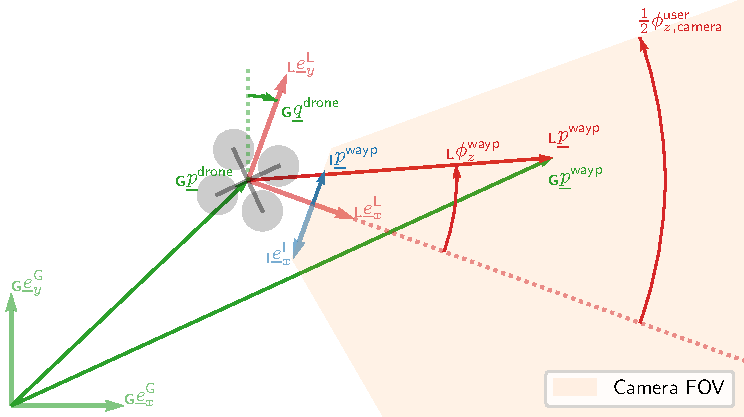
\includegraphics[width=0.9\textwidth]{own/global_via_local_to_image_transformation_2d.pdf}
%    \caption[
%        Schematic 2D depiction
%        of the transformation of the waypoint 
%        from the global via the local to the image reference system.
%    ]{
%        Schematic 2D depiction
%        of the transformation of the waypoint 
%        from the global ${}_\textbf{G}\square$ 
%        via the local ${}_\textbf{L}\square$ 
%        to the image ${}_\textbf{I}\square$ reference system.
%        Unit vectors 
%        $\underline e_\square \in \mathbb{R}^3,\ \left\|\underline e_\square \right\|_2 = 1$ 
%        spanning the individual reference systems,
%        points $\underline p^\square \in \mathbb{R}^3$,
%        quaternions $\underline q^\square \in \mathbb{R}^4$
%        and angles $\phi_\square^\square  \in \mathbb{R}$
%        relative to the global, local or image reference system
%        are colored in green, red or blue, respectively.
%        %Unit vectors are drawn
%        %with a greater linewidth and lower opacity 
%        %than the positions, quaternions and angles.
%        The z unit vectors 
%        ${}_\textbf{G} e^\text{G}_z$
%        and
%        $\ {}_\textbf{L} e^\text{L}_z$ 
%        of the global and local reference system,
%        the y unit vector 
%        ${}_\textbf{I} e^\text{I}_y$ 
%        of the image reference system
%        and the pitch angle 
%        $\phi^\text{user}_{y,\text{camera}}$
%        of view of the camera
%        are not pictured
%        in this 2D representation.
%        %but point in the direction of the reader.
%        The field of view (FOV) of the onboard camera of the drone
%        is marked with a low-opaque orange.
%
%        The global position
%        ${}_\textbf{G}\underline p^\text{drone}$
%        and quaternion orientation
%        ${}_\textbf{G}\underline q^\text{drone}$
%        of the drone,
%        the yaw
%        $\phi^\text{user}_{z,\text{camera}}$
%        and pitch
%        $\phi^\text{user}_{y,\text{camera}}$ 
%        angle of view of the camera
%        as well as the global position of the waypoint
%        ${}_\textbf{G}\underline p^\text{wayp}$
%        are known.
%        First, the local position of the waypoint
%        ${}_\textbf{L}\underline p^\text{wayp}$
%        is computed by applying the transformation
%        $T_\textbf{LG}$
%        (equation \ref{equ:global_to_local_transformation}).
%        Second, 
%        ${}_\textbf{L}\underline p^\text{wayp}$
%        is transformed with 
%        $T_\textbf{IL}$
%        (equation \ref{equ:local_to_image_transformation})
%        yielding 
%        the position of the waypoint
%        ${}_\textbf{I}\underline p^\text{wayp}$ 
%        with respect to the image reference system.
%        $T_\textbf{LG}$ is fully determined by 
%        ${}_\textbf{G}\underline p^\text{drone}$ 
%        and 
%        ${}_\textbf{G}\underline q^\text{drone}$.
%        $T_\textbf{IL}$ is fully determined by
%        $\phi^\text{user}_{z,\text{camera}}$
%        and
%        $\phi^\text{user}_{y,\text{camera}}$.
%        \label{fig:trafo}
%    }
%\end{figure}



\section{ANN module} \label{sec:ann_module}
The ANN module performs the function of inference
within the autonomous navigation method.
More precisely, the module makes navigation decisions
on the basis of data from the drone's onboard sensors.
In order for these navigation decisions to be reasonable
the ANN module is trained with supervised learning (see section ??).
At testing, 
when the autonomous navigation method flies the drone through the racetrack,
the ANN module outputs navigation decisions in real-time at a user-specified frequency.
Thereby, the GRU sub-module (and therewith the ANN module itself)
operates in one-to-one mode,
i.e., it maps each single, non-sequential input to a single, non-sequential output.
As, however, the frequently incoming, single inputs as a whole constitute a time series,
the GRU sub-module builds up memory in its hidden state
as the module learned during training.
By this, not only the current but also 
past inputs have impact on the current navigation decision.


The ANN module itself is built 
from the CNN, the CAT, the GRU, the FC and the HEAD sub-module
(see figure XXX).
This modular design entails a high flexibility for the studies
of different ANN module variants in chaper ??.
For all ANN module variants,
the sequence of the sub-modules is fixed
and the outer sub-modules, i.e, the CNN and the HEAD sub-module,
are mandatory.
This ensures the mapping 
of the minimum input of an RGB image to a navigation decision.
In contrast, the user specifies whether
the individual inner sub-modules,
i.e., the CAT, the GRU and the FC sub-module,
are switched on or off
before the training of an ANN module variant.
Moreover, the user specifies the design of all individual sub-modules.



\paragraph*{Input} ${}$\\
The single inputs to the ANN module are devided into mandatory and optional.
The mandatory input for the current inference is the
latest, preprocessed RGB (therewith three channeled) image from the drone's onboard camera
\begin{equation}
    \underline{\underline{\underline I}}^\text{preproc}
    \in 
    %\left\{
    %    0,\dots,I_\text{max}
    %\right\}
    \left\{
        \frac{i}{I_\text{max}^\text{raw}}
    \right\}
    _{
        i \in 
        \left\{
            0,\dots,I_\text{max}^\text{raw}
        \right\}
    }
    ^{
        %I_\text{C} \times    
        3 \times
        I_\text{H}^\text{preproc} \times 
        I_\text{W}^\text{preproc}
    }.
    %\text{ with } I_\text{C} = 3.
\end{equation}
The two-step preprocessing of the raw RGB image simplifies the training of the ANN module.
First, the pixel intensities are normalized by the full intensity 
$I_\text{max}^\text{raw} = 255$
with the aim to accelerate the convergence at training.
Second, the image is sized down 
to the height 
$
    I_\text{H}^\text{preproc} 
    = 
    \left\lfloor
    s^\text{user}_\text{rgb-resize}
    \cdot
    I_\text{H}^\text{raw}
    \right\rfloor
$
and width
$
    I_\text{W}^\text{preproc} 
    = 
    \left\lfloor
    s^\text{user}_\text{rgb-resize}
    \cdot
    I_\text{W}^\text{raw}
    \right\rfloor
$
with a user-specified 
factor preserving its aspect ratio.
By this, the occupation of GPU memory at training,
which is critical for longer sequences,
can be reduced if necessary.



Before the training of an ANN module variant, the user switches on or off
the individual elements of the feature vector of optional inputs
\begin{align}
    \featvec[]{\text{opt}}{}{}{} 
    =
    \begin{bmatrix}
        \dur[]{\text{rgb}}{}{}{} \\
        \acc[\hat]{\text{imu}}{}{}{} \\
        \angvel[\hat]{\text{imu}}{}{}{} \\
        \dur[]{\text{imu}}{}{}{}
    \end{bmatrix}
    .
\end{align}
The above vector comprises the
the duration
$\dur[]{\text{rgb}}{}{}{}$
elapsed between the shooting of the previous and the latest raw RGB image,
the drone's latest linear acceleration
$\acc[\hat]{\text{imu}}{}{}{} \in \mathbb{R}^3$
and angular velocity
$\angvel[\hat]{\text{imu}}{}{}{} \in \mathbb{R}^3$
measurement from its onboard inertial measurement unit (IMU)
as well as the duration
$\dur[]{\text{imu}}{}{}{}$
elapsed between the recording of the previous and the latest IMU data.








\subsection*{CNN}
The convolutional neural network (CNN) sub-module
extracts a batch of visual features 
from the pixel data of a batch of images
\begin{align} \label{eq:CNN}
    \underline{\underline{ \mathcal{F} }}^\text{cnn}
    :\ 
    & 
    \mathbb{R}^{
        N^\text{cnn}_\text{batch} 
        \times
        N^\text{cnn}_\text{channel}
        \times
        N^\text{cnn}_\text{height}
        \times
        N^\text{cnn}_\text{width}
    } 
    \rightarrow 
    \mathbb{R}^{
        N^\text{cnn}_\text{batch}
        \times
        N^\text{cnn}_\text{out}
    }
    \nonumber \\
    %;\quad
    &\underline{\underline{\underline{\underline x}}}
    \mapsto 
    \underline{\underline{ \mathcal{F} }}^\text{cnn} \left(
        \underline{\underline{\underline{\underline x}}}
    \right)
    .
\end{align}
The batch size 
$
    N^\text{cnn}_\text{batch}
$,
the number of channels
$
    N^\text{cnn}_\text{channel}
$
as well as the image height 
$
    N^\text{cnn}_\text{height}
$
and width
$
    N^\text{cnn}_\text{width}
$
of the CNN
adapt to the dimensions of the inputted batch of images
$
    \underline{\underline{\underline{\underline x}}}
$,
whereas the output size
$
    N^\text{cnn}_\text{out}
$
of the CNN
is fixed by the design of the CNN, 
more specifically, by its last layer.
The training data is generally sequential,
i.e., the images are present in batches of sequences
\begin{equation}
    \underline{\underline{\underline{\underline{\underline x}}}} ^\text{rgb}
    \in
    \mathbb{R}^{
        N^\text{batch} 
        \times
        N^\text{seq}
        \times
        N^\text{C}
        \times
        N^\text{H}
        \times
        N^\text{W}
    }
\end{equation}
with the sequence lenght $N^\text{seq}$.
These batches of sequences must be
vectorized along their two first dimensions
\begin{equation}
    \mathrm{vec} \left(
        \underline{\underline{\underline{\underline{\underline x}}}} ^\text{rgb}   
    \right)
    \in
    \mathbb{R}^{
        N^\text{batch} 
        \cdot
        N^\text{seq}
        \times
        N^\text{C}
        \times
        N^\text{H}
        \times
        N^\text{W}
    }
\end{equation}
before they are processed by the CNN.
Afterwards the sequences are restored 
by de-vectorizing the direct output of the CNN backbone 
\begin{equation}
    \underline{\underline{\underline{x}}}^\text{cnn}
    =
    \mathrm{vec}^{-1} \left(
        \underline{\underline{ \mathcal{F} }}^\text{cnn} \left(
            \mathrm{vec} \left(
                \underline{\underline{\underline{\underline{\underline x}}}} ^\text{rgb}   
            \right)
        \right)
    \right)
    \in
    \mathbb{R}^{
        N^\text{batch} 
        \times
        N^\text{seq}
        \times
        N^\text{cnn}_\text{out}
    }.
\end{equation}

\subsection*{CAT}
The CAT sub-module concatenates
each corresponding pair of sequential feature matrices,
sampled from 
the
batch outputted by the CNN sub-module
and the batch of optional inputs,
along their feature axis
\begin{align} \label{eq:cat}
    \mathcal{F}^\text{cat}
    :\ 
    & \left(
        \mathbb{R}^{
            N^\text{seq}
            \times
            N^\text{cnn}_{\text{out}}
        }
        ,\ 
        \mathbb{R}^{
            N^\text{seq}
            \times
            N^\text{input}_{\text{opt}}
        }
    \right)
    \rightarrow 
    \mathbb{R}^{
            N^\text{seq}
            \times
            \left(
                N^\text{cnn}_{\text{out}}
                + 
                N^\text{input}_{\text{opt}}
            \right)
        }
    \nonumber \\ &
    \left(
        \underline{\underline{x}}_{i}
        ,\ 
        \underline{\underline{y}}_{i}
    \right)
    \mapsto
    \begin{bmatrix}
        \underline{\underline{x}}_{i} & \underline{\underline{y}}_{i}
    \end{bmatrix} 
    ,\qquad
    i \in \left\{
        1, \dots, N^\text{batch}
    \right\}.
\end{align}
If the user deactivates all optional input, i.e.,
$
    N^\text{input}_{\text{opt}} = 0
$,
the CAT sub-module recedes to 
the identity map
of the output of the CNN sub-module.
Either way, 
the CAT sub-module has zero trainable parameters
\begin{equation}
    N^\text{cat}_\text{param} = 0.
\end{equation}


%The user specifies a subset of all possible optional inputs.
\subsection*{GRU}
The GRU sub-module consists of multiple layers of 
gated recurrent units (GRU) \cite{Cho2014}.
%RNN

The input to a single unit is
a batch of sequences of feature vectors
\begin{equation}
    \left(
        \underline x_k
    \right)_{
        k \in \left\{
            1, \dots, N^\text{seq}
        \right\}
        ,
        j
    }
    ,\quad
    j \in \left\{
        1, \dots, N^\text{batch}
    \right\}
\end{equation}
and a batch of the hidden states
previously inferenced by the unit
\begin{equation}
    \underline h_{0,j}
    ,\quad
    j \in \left\{
        1, \dots, N^\text{batch}
    \right\}.
\end{equation}


-----------------------

The $i$-th gated recurrent unit 
%$
%    i 
%    \in 
%    \left\{
%        1, \dots, N^\text{gru}_\text{unit}
%    \right\}
%$
maps the $k$-th feature vector of
the $j$-th sequence 
%$
%    j 
%    \in 
%    \left\{
%        1, \dots, N^\text{batch}
%    \right\}
%$
of its input batch, i.e.,
$\underline x_{k,j}$,
and the $j$-th previous hidden state
of its hidden batch,
i.e., $\underline h_{k-1,j}$,
to the $j$-th current hidden state of its output batch,
i.e., $\underline h_{k,j}$,
by averaging
its new gate 
$\mathcal{F}^\text{gru}_{\text{new},i}$
and its previous hidden state,
weighted with its update gate
$\mathcal{F}^\text{gru}_{\text{upd},i}$
\begin{align} \label{eq:gru_hidden}
    \forall \quad &
    i \in \left\{
        1, \dots, N^\text{gru}_\text{unit}
    \right\}
    ,\ 
    j \in \left\{
        1, \dots, N^\text{batch}
    \right\}
    ,\ 
    k \in \left\{
        1, \dots, N^\text{seq}
    \right\}
    :
    \nonumber \\ &
    \mathcal{F}^\text{gru}_{\text{hidden},i}
    :\
    \left(
        \mathbb{R}^{
            N^\text{gru}_{\text{in}, i}
        }
        ,\ 
        \left[
            -1, 1
        \right]^{
            N^\text{gru}_{\text{hidden}}
        }
    \right)
    \rightarrow 
    \left[
        -1, 1
    \right]^{
        N^\text{gru}_{\text{hidden}}
    }
    \nonumber \\ & \quad
    \chi
    :=
    \left(
        \underline x_{k,j}
        ,\ 
        \underline h_{k-1,j}
    \right)
    \mapsto
    \nonumber \\ & \qquad \qquad
    \underline h_{k,j}
    =
    \left[
        1 
        -
        \mathcal{F}^\text{gru}_{\text{upd},i} \left(
            \chi
        \right)
    \right]
    \odot
    \mathcal{F}^\text{gru}_{\text{new},i} \left(
        \chi
    \right)
    %\nonumber \\ & \qquad 
    +
    \mathcal{F}^\text{gru}_{\text{upd},i} \left(
        \chi
    \right)
    \odot
    \underline h_{k-1,j}
    .
\end{align}
In addition to the update and new gate,
a gated recurrent unit also incorporates
the reset gate which is used to compute the new gate.
These three gates
follow the mappings
\begin{align} \label{eq:gru_reset}
    \forall \quad &
    i \in \left\{
        1, \dots, N^\text{gru}_\text{unit}
    \right\}
    ,\ 
    j \in \left\{
        1, \dots, N^\text{batch}
    \right\}
    ,\ 
    k \in \left\{
        1, \dots, N^\text{seq}
    \right\}
    :
    \nonumber \\ &
    \mathcal{F}^\text{gru}_{\text{reset},i}
    ,\ 
    \mathcal{F}^\text{gru}_{\text{upd},i}
    ,\ 
    \mathcal{F}^\text{gru}_{\text{new},i}
    :\
    \left(
        \mathbb{R}^{
            N^\text{gru}_{\text{in},i}
        }
        ,\ 
        \left[
            -1, 1
        \right]^{
            N^\text{gru}_{\text{hidden}}
        }
    \right)
    \rightarrow
    \left[
        0, 1   
    \right]^{
        N^\text{gru}_{\text{hidden}}
    }
    ,\ 
    \left[
        0, 1   
    \right]^{
        N^\text{gru}_{\text{hidden}}
    },\ 
    \left[
        -1, 1   
    \right]^{
        N^\text{gru}_{\text{hidden}}
    }
    \nonumber \\ & \quad
    \chi
    :=
    \left(
        \underline x_{k,j}
        ,\ 
        \underline h_{k-1,j}
    \right)
    \mapsto
    \nonumber \\ & \qquad\qquad
        \sigma \fullmoon \left(
            \underline{\underline A}^\text{reset}_{x,i}
            \underline x_{k,j}
            +
            \underline b^\text{reset}_{x,i}
            +
            \underline{\underline A}^\text{reset}_{h,i}
            \underline h_{k-1,j}
            +
            \underline b^\text{reset}_{h,i}
        \right)
    ,
    \nonumber \\ & \qquad\qquad
        \sigma \fullmoon \left(
            \underline{\underline A}^\text{upd}_{x,i}
            \underline x_{k,j}
            +
            \underline b^\text{upd}_{x,i}
            +
            \underline{\underline A}^\text{upd}_{h,i}
            \underline h_{k-1,j}
            +
            \underline b^\text{upd}_{h,i}
        \right)
    ,
    \nonumber \\ & \qquad\qquad
        \tanh \fullmoon \left[
            \underline{\underline A}^\text{new}_{x,i}
            \underline x_{k,j}
            +
            \underline b^\text{new}_{x,i}
            %\nonumber \\ & \qquad \qquad \qquad \qquad \qquad \qquad \quad 
            +
            \mathcal{F}^\text{gru}_\text{reset} \left(
                \chi
            \right)
            \odot
            \left(
                \underline{\underline A}^\text{new}_{h,i}
                \underline h_{k-1,j}
                +
                \underline b^\text{new}_{h,i}
            \right)
        \right]
    .
\end{align}
The reset gate linearly transforms the feature vector and the previous hidden state
with the matrices of trainable weights and the vectors of trainable biases
\begin{align}
    \underline{\underline A}^\text{reset}_{x,i}
    &\in \mathbb{R}^{
        N^\text{gru}_{\text{hidden}}
        \times
        N^\text{gru}_{\text{in},i}
    }
    ,
    &\underline{\underline A}^\text{reset}_{h,i}
    &\in \mathbb{R}^{
        N^\text{gru}_{\text{hidden}}
        \times
        N^\text{gru}_{\text{hidden}}
    }
    ,
    \nonumber \\
    \underline{b}^\text{reset}_{x,i}
    &\in \mathbb{R}^{
        N^\text{gru}_{\text{hidden}}
    }
    ,
    &\underline{b}^\text{reset}_{h,i}
    &\in \mathbb{R}^{
        N^\text{gru}_{\text{hidden}}
    }
    ,
\end{align}
and applies the standard sigmoid function \cite{Han1995}
\begin{equation}
    \sigma
    :\ 
    \mathbb{R}
    \rightarrow
    \left[
        0,1
    \right]
    ;\ 
    x \mapsto \frac{1}{1 + e^{-x}}
\end{equation}
elementwise (denoted with $\fullmoon$) to the result.
The update gate differs to the reset gate only in the fact
that it has own trainable weights and biases
\begin{align}
    \underline{\underline A}^\text{upd}_{x,i}
    &\in \mathbb{R}^{
        N^\text{gru}_{\text{hidden}}
        \times
        N^\text{gru}_{\text{in},i}
    }
    ,
    &\underline{\underline A}^\text{upd}_{h,i}
    &\in \mathbb{R}^{
        N^\text{gru}_{\text{hidden}}
        \times
        N^\text{gru}_{\text{hidden}}
    }
    ,
    \nonumber \\
    \underline{b}^\text{upd}_{x,i}
    &\in \mathbb{R}^{
        N^\text{gru}_{\text{hidden}}
    }
    ,
    &\underline{b}^\text{upd}_{h,i}
    &\in \mathbb{R}^{
        N^\text{gru}_{\text{hidden}}
    }
    .
\end{align}
The new gate also linearly transforms the feature vector and the previous hidden state
with its own weights and biases
\begin{align}
    \underline{\underline A}^\text{new}_{x,i}
    &\in \mathbb{R}^{
        N^\text{gru}_{\text{hidden}}
        \times
        N^\text{gru}_{\text{in},i}
    }
    ,
    &\underline{\underline A}^\text{new}_{h,i}
    &\in \mathbb{R}^{
        N^\text{gru}_{\text{hidden}}
        \times
        N^\text{gru}_{\text{hidden}}
    }
    ,
    \nonumber \\
    \underline{b}^\text{new}_{x,i}
    &\in \mathbb{R}^{
        N^\text{gru}_{\text{hidden}}
    }
    ,
    &\underline{b}^\text{new}_{h,i}
    &\in \mathbb{R}^{
        N^\text{gru}_{\text{hidden}}
    }
    .
\end{align}
In contrast to the other two gates,
the new gate, before building the sum of both linear transformations,
mitigates the contribution of the linear transformation of the 
hidden state by the Hadamard product with the reset gate.
Moreover, the hyperbolic tangent \cite{D.1966}
\begin{equation}
    \tanh
    :\ 
    \mathbb{R}
    \rightarrow
    \left[
        -1,1
    \right]
    ;\ 
    x 
    \mapsto 
    \frac{
        e^x - e^{-x}
    }{
        e^x + e^{-x}
    }
\end{equation}
and not the sigmoid function 
is applied element-wise.



applies the following maps
For the computation of the current batch of hidden states,
the unit intermittently maps its input to three gates.
The reset gate is computed by 
applying the sigmoid function
$
\sigma(x) = \frac{1}{1+\exp(-x)}
$
to the individual elements of the sum
of the biased linear transformations
to the inputs and the previous hidden states
and the subsequent


This multi-layer gated recurrent unit (GRU)
uses feedback connection to process the time series data
thereby inttroducing temporal understanding in the decision making.



\subsection*{FC}
The FC sub-module comprises multiple fully connected layers
applied to a batch of features.
Each layer 
$
    i 
    \in 
    \left\{
        1, \dots, N^\text{fc}_\text{layer}
    \right\}
$ 
applies
an activation function,
a dropout
and a biased linear transformation
on each element
$
    j
    \in 
    \left\{
        1, \dots, N^\text{batch}
    \right\}
$
of a batch
\begin{align} \label{eq:FC}
    \mathcal{F}^\text{fc}_i
    :\ &
    \mathbb{R}^{
        %N^\text{batch} 
        %\times
        N^\text{fc}_{\text{in}, i}
    }
    \rightarrow 
    \mathbb{R}^{
            %N^\text{batch} 
            %\times
            N^\text{fc}_\text{out}
        }
    \nonumber \\ &
    %;\quad
    \underline{x}_j%^\text{fc}_\text{in}
    \mapsto
    %\underline{\underline{x}}^\text{fc}_\text{out}
    %=
    \underline{\underline A}^\text{fc}_i
    \left(
        \underline{\delta}^\text{fc}
        \odot
        f^\text{fc} \fullmoon \left(
            \underline{x}_j%^\text{fc}_\text{in}
        \right)
    \right)
    + \underline b^\text{fc}_i
    %
    %\nonumber \\ &
    %x_{kl}
    %\mapsto
    %\sum_l \delta_{kl} f(x_{kl}) a_{lm} + b_m 
    .
\end{align}
The activation function 
$
    f^\text{fc}: \mathbb{R} \rightarrow \mathbb{R}
$
is applied element-wise (denoted with $\fullmoon$) on the input
and is chosen by the user from the non-linear activations
provided by PyTorch\footnote{
    \url{https://pytorch.org/docs/stable/nn.html}, visited on 03/07/2022
}.
The dropout\cite{Hinton2012} decreases the overfitting of the ANN module on the training data set
by enforcing the neurons to learn the detection of stand-alone features
whose informative value is independent from
the relation to other detected features.
The dropout is accomplished
by the Hadamard product (denoted with $\odot$)
with the vector
\begin{equation}
    \underline{\delta}^\text{fc}
    =
    \left[
        \delta^\text{fc}_i
    \right]_{
        i \in \left\{
            1, \dots, N^\text{fc}_{\text{in}, i}
        \right\}
    }
\end{equation}
of independent, scaled Bernoulli random variables
that are resampled for every function call
with the probabilities
\begin{equation}
    P \left(
        \delta^\text{fc}_i = 0
    \right)
    = p^\text{fc}
    ,\quad
    P \left(
        \delta^\text{fc}_i = \frac{1}{1-p^\text{fc}}
    \right)
    = 1 - p^\text{fc}
    .
\end{equation}
During training,
the dropout probability $p^\text{fc} \in [0,1]$ equates to value specified by the user,
whereas during evaluation,
it is null $p^\text{fc} = 0$
whereby the dropout becomes an identity operation.
The linear transformation
consist of the linear map given by the matrix of trainable weights
\begin{equation}
    \underline{\underline A}^\text{fc}_i 
    \in 
    \mathbb{R}^{
        N^\text{fc}_{\text{in}, i}
        \times
        N^\text{fc}_\text{out}
    }
\end{equation}
and the addition of the vector of trainable biases
\begin{equation}
    \underline b^\text{fc}_i 
    \in \mathbb{R}^{
        N^\text{fc}_\text{out}
    }.
\end{equation}
A single layer, thus,
has
$
    \left(
        N^\text{fc}_{\text{in}, i} + 1
    \right)
    \cdot
    N^\text{fc}_\text{out}
$
trainable parameters.
The user specifies the number of layers
$
    N^\text{fc}_\text{layer}
$
of the FC, the width 
$
    N^\text{fc}_\text{out}
$,
i.e., the number of outputted features,
which is shared by all layers of the FC,
the activation function 
$
    f^\text{fc}: \mathbb{R} \rightarrow \mathbb{R}
$
and the dropout probability
$
    p^\text{fc} \in [0,1]
$.
The number of inputted features
of a layer
adapts to the given input
$
    N^\text{fc}_{\text{in}, i} 
    = 
    \begin{cases}
        \dim \left(
            \underline{x}_j
        \right)
        ,\quad 
        \text{if } i = 1
        \\
        N^\text{fc}_\text{out}
        ,\quad 
        \text{else} 
    \end{cases}
$.
For 
$
    N^\text{fc}_\text{layer} \ge 1
$,
the FC sub-module hence has
a total of 
$
    \left(
        N^\text{fc}_{\text{in}, i} + 1
    \right)
    %\cdot
    N^\text{fc}_\text{out}
    +
    \left(
        N^\text{fc}_\text{layer} - 1
    \right)
    %\cdot
    \left(
        N^\text{fc}_\text{out} + 1
    \right)
    %\cdot
    N^\text{fc}_\text{out}
$
trainable parameters.

\subsection*{HEAD}
The HEAD sub-module is mandatory
since it produces 
the final output of the entire ANN module
which is,
depending on the user's selection,
either a navigation decision
or a control command.
A navigation decision 
\begin{equation} \label{eq:navigation_decision}
    (
        v_\text{norm},
        \ 
        {}_\textbf{I} \underline p^\text{wayp}
    )   
\end{equation}
consists of a normalized speed 
$v_\text{norm} \in [0, 1]$
and a waypoint
${}_\textbf{I} \underline p^\text{wayp} \in [-1, 1]^2$
in the image reference system
(see figure \ref{fig:image_reference_system}).
A control command 
\begin{equation}
    (
        {}_\textbf{I} \underline \omega^\text{cmd},\ 
        {}_\textbf{I} \underline{\dot\omega}^\text{cmd},\ 
        c^\text{cmd}
    )
\end{equation}
comprises the desired angular velocity
${}_\textbf{I} \underline \omega^\text{cmd}$
(also referred to as body rates)
and acceleration
$
{}_\textbf{I} \underline{\dot\omega}^\text{cmd}
$
of the drone body
as well as the desired collective thrust 
$c^\text{drone}$
of the drone rotors.
In the limited scope of this master's thesis,
the option to output control commands
is only implemented but not tested in experiments.
The mapping of the HEAD entails 
an activation function and a biased linear transformation
which are deployed to each feature vector
of the input batch
\begin{align} \label{eq:head}
    \mathcal{F}^\text{head}
    :\ &
    \mathbb{R}^{
        N^\text{head}_\text{in}
    }
    \rightarrow 
    \mathbb{R}^{
            N^\text{head}_\text{out}
        }
    \nonumber \\ &
    \underline{x}_j
    \mapsto
    \underline{\underline A}^\text{head}
    \left(
        f^\text{head} \fullmoon \left(
            \underline{x}_j
        \right)
    \right)
    + \underline b^\text{head}
    ,\quad
    j
    \in 
    \left\{
        1, \dots, N^\text{batch}
    \right\}
    .
\end{align}
This structure is similar to a layer of the FC sub-module
(see equation \ref{eq:FC}),
leaving out the dropout functionality.
While the number of input features is adaptive
\begin{equation}
    N^\text{head}_\text{in}
    =
    \dim \left(
        \underline{x}_j
    \right),
\end{equation}
the number of output features is determined by 
the user-selected output
\begin{equation}
    N^\text{head}_\text{out}
    = 
    \begin{cases}
        3
        ,\quad 
        \text{if navigation decision} 
        \\
        7
        ,\quad 
        \text{if control command} 
    \end{cases}.
\end{equation}
The total number of trainable parameters of the HEAD sub-module is
\begin{equation}
    N^\text{head}_\text{params} 
    = 
    \left(
        N^\text{head}_\text{in} + 1
    \right)
    %\cdot
    N^\text{head}_\text{out}
\end{equation}


\subsection{Baseline config}



%CNN: torch vision model, pretrained, trainable, adapt to any RGB size
%CAT: CNN output , CAT input , one vector
%GRU: hidden size, num_layers, bias, dropout
%FC: width, num_layers, act fct, bias
%HEAD: output size, act fct, bias
%GRAPH
%
%loss optimizer learnrate


-resize image dims by a factor
-cnn backbone
-cat cnn output with optional inputs
-multilayer gru if data sequential
-multilayer fc
-head




\subsection*{Output}










\section{Planning module}
The planning module performs the task of path planning
within the autonomous navigation method.
At the user-specified main frequency 
$\freq[\user]{\main}{}{}{}$,
the planning module 
samples states from its local trajectory
and forwards them as reference to the control module.
Every $\num[\user]{\text{plan}}{}{}{}$-th (user-specified) iteration,
the planning module re-computes its local trajectory
on the basis of its input,
i.e., the latest navigation decision and the latest drone state estimate. 
%These trajectories, generated by the planning module, 
%are referred to as local trajectories
%to distinguish them from the expert system's global trajectory
%used when generating training data for the ANN module (see XX).

The latest navigation decision
stems from either the ANN module
(see equ. \ref{eq:navigation_decision}) 
or, if it has intervened at training data generation,
the expert system (see equ. \ref{eq:nav_dec_by_expert}).
A navigation decision comprises the normalized desired speed 
and the waypoint in the image reference system
\begin{equation}
    (
        \speed[\norm]{\drone}{\desired}{}{}
        ,\ 
        \pos[]{\wayp}{}{\irs}{}
    ).
\end{equation}
The latest drone state estimate stems from the state estimation system.
In simulation, the estimate may correspond to the ground-truth state.
A drone state estimate includes position, velocity and acceleration
with respect to the global reference system
\begin{equation} \label{eq:drone_state}
    \pos[]{\drone}{}{\grs}{}
    ,\ 
    \vel[]{\drone}{}{\grs}{}
    ,\ 
    \acc[]{\drone}{}{\grs}{}.
\end{equation}


At a fraction of the main frequency, i.e.,
$\freq[\user]{\main}{}{}{} / \num[\user]{\text{plan}}{}{}{}$, 
the planning module takes the following 5 steps 
to re-compute its local trajectory.
\begin{enumerate}
    \item Compute the desired speed
    \begin{equation}
        \speed[]{\drone}{\desired}{}{}
        = 
        \maxof{
            \speed[\user]{\drone}{\mnm}{}{}
        }{
            \speed[\user]{\drone}{\mxm}{}{}
            \cdot 
            \speed[\norm]{\drone}{\desired}{}{}
        }.
    \end{equation}
    The normalized, desired speed 
    $\speed[\norm]{\drone}{\desired}{}{} \in \left[0, 1\right]$ 
    of the navigation decision
    is rescaled by its upper bound, 
    the user-specified drone's maximum speed 
    $\speed[\user]{\drone}{\mxm}{}{}$.    
    The user-specified drone's minimum speed 
    $\speed[\user]{\drone}{\mnm}{}{}$
    lower-bounds the desired speed.

    \item Compute the drone's distance to the waypoint 
    \begin{equation}
        \dist[]{\dronetowayp}{}{}{}
        = 
        \maxof{
            \dist[\user]{\dronetowayp}{\mnm}{}{}
        }{
            \minof{
                \speed[]{\drone}{\desired}{}{}
                \cdot
                \dur[\user]{\dronetowayp}{}{}{}
            }{
                \dist[\user]{\dronetowayp}{\mxm}{}{}
            }
        }.
    \end{equation}
    The desired speed 
    $\speed[]{\drone}{\desired}{}{}$ 
    is integrated over the user-specified duration
    $\dur[\user]{\dronetowayp}{}{}{}$.
    The result is bounded to the interval spanned 
    by the user-specified minimum
    $\dist[\user]{\dronetowayp}{\mnm}{}{}$
    and maximum
    $\dist[\user]{\dronetowayp}{\mxm}{}{}$
    distance.

    \item Compute the waypoint with respect to the global reference system
    \begin{equation} \label{eq:pl_global_wayp}
        \pos[]{\wayp}{}{\grs}{}
        = 
        \trafo[]{}{\grs\irs}{}{} \left(
            \dist[]{\dronetowayp}{}{}{}
            ,\ 
            \pos[]{\wayp}{}{\irs}{}
        \right).
    \end{equation}
    The transformation
    $\trafo[]{}{\grs\irs}{}{}$
    (see equ. \ref{eq:global_image_transformations})
    backprojects the waypoint
    $\pos[]{\wayp}{}{\irs}{}$ 
    of the navigation decision
    from the 2D image to the 3D global reference system.
    Thereby, the drone's distance 
    $\dist[]{\dronetowayp}{}{}{}$
    to the waypoint
    constitutes the backprojection length.
    
    \item Set the starting time of the local trajectory to the current time
    \begin{equation}
        \timepnt[]{\loctraj}{0}{}{} = t
    \end{equation}
    and compute the duration of the local trajectory 
    \begin{equation}
        \dur[]{\loctraj}{}{}{}
        = 
        \frac{
            \dist[]{\dronetowayp}{}{}{}
        }{
            \minof{
            \speed[]{\drone}{\desired}{}{}
            }{
                %\speed[]{\drone}{}{}{} 
                \left\|
                    \vel[]{\drone}{}{\grs}{}
                \right\|_2
                + 
                \speed[\user]{\drone}{\Delta}{}{}
            }
        }.
    \end{equation}
    The drone's distance 
    $\dist[]{\dronetowayp}{}{}{}$
    to the waypoint is devided 
    by the slower of either the desired speed
    $\speed[]{\drone}{\desired}{}{}$
    or the latest drone speed estimate
    $\left\|\vel[]{\drone}{}{\grs}{}\right\|_2$
    plus a user-specified speed increment
    $\speed[\user]{\drone}{\Delta}{}{}$.
    By relating the desired to the estimated speed,
    excessive speed increases
    potentially violating the drone's dynamic limitations
    can be prevented.

    \item Compute the local trajectory 
    \begin{align} \label{eq:loc_traj}
        \pos[]{\loctraj}{}{\grs}{}
        :\ 
        &\left[0, \dur[]{\loctraj}{}{}{}\right] \rightarrow \mathbb{R}^3
        ;\quad
        %\nonumber \\
        \timepnt[]{}{}{}{}
        \mapsto
        \pos[]{\loctraj}{}{\grs}{}(\timepnt[]{}{}{}{})
    \end{align}
    starting in the latest drone state estimate
    $\pos[]{\drone}{}{\grs}{}
    ,\ 
    \vel[]{\drone}{}{\grs}{}
    ,\ 
    \acc[]{\drone}{}{\grs}{}$
    and ending in the global waypoint
    $\pos[]{\wayp}{}{\grs}{}$
    with unconstrained velocity and acceleration.
    The implementation\footnote{
            \url{https://github.com/markwmuller/RapidQuadrocopterTrajectories}, visited on 17/08/2022
    } 
    of the algorithm of Mueller et. al. \cite{Mueller2013}
    is deployed to find the polynomial trajectory with minimum jerk
    (third time derivative of position)
    by solving the optimization problem
    \begin{align}
        &\qquad \min 
        \int_0^{\dur[]{\loctraj}{}{}{}}
            \left\|
                \pos[\dddot]{\loctraj}{}{\grs}{}(\timepnt[]{}{}{}{})
            \right\|^2_2
        \text d \timepnt[]{}{}{}{}
        \nonumber \\
        \text{s.t.}\quad
        & \pos[]{\loctraj}{}{\grs}{}(0) = \pos[]{\drone}{}{\grs}{}
        \qquad\qquad \pos[]{\loctraj}{}{\grs}{}(\dur[]{\loctraj}{}{}{}) = \pos[]{\wayp}{}{\grs}{}
        \nonumber \\
        & \pos[\dot]{\loctraj}{}{\grs}{}(0) = \vel[]{\drone}{}{\grs}{}
        \qquad\qquad \pos[\dot]{\loctraj}{}{\grs}{}(\dur[]{\loctraj}{}{}{}) \text{ free}
        \nonumber \\
        & \pos[\ddot]{\loctraj}{}{\grs}{}(0) = \acc[]{\drone}{}{\grs}{}
        \qquad\qquad \pos[\ddot]{\loctraj}{}{\grs}{}(\dur[]{\loctraj}{}{}{}) \text{ free}.
    \end{align}
    The drone's dynamic limitations
    are only taken into account in subsequent feasibility checks 
    and are exempt from the above optimization problem.
    This allows the algorithm to solve the optimization problem in closed form
    which is characterized by low computational effort.
    The algorithm therewith qualifies 
    to run at the relatively high frequencies
    required by the autonomous navigation method.
\end{enumerate}


At the main frequency $\freq[\user]{\main}{}{}{}$, 
the planning module takes the following 2 steps to sample 
a reference state from its local trajectory.
\begin{enumerate}
    \item Compute the time point of the reference state
    \begin{equation}
        \timepnt[]{\loctraj}{}{}{} 
        = 
        t - \timepnt[]{\loctraj}{0}{}{} + 1/\freq[\user]{\main}{}{}{}.
    \end{equation}
    The actual time $t$ is related to the starting time 
    $\timepnt[]{\loctraj}{0}{}{}$
    of the local trajectory,
    whose time domain starts at zero.
    The addition of the main period
    $1/\freq[\user]{\main}{}{}{}$
    ensures that the sampled reference state remains prospective at all times.
    \item Sample the current reference state from the local trajectory
    \begin{align} \label{eq:ref_state}
        \pos[]{\text{ref}}{}{\grs}{} 
        &= 
        \pos[]{\loctraj}{}{\grs}{}(\timepnt[]{\loctraj}{}{}{})
        \nonumber \\
        \vel[]{\text{ref}}{}{\grs}{} 
        &= 
        \pos[\dot]{\loctraj}{}{\grs}{}(\timepnt[]{\loctraj}{}{}{})
        \nonumber \\
        \acc[]{\text{ref}}{}{\grs}{} 
        &= 
        \pos[\ddot]{\loctraj}{}{\grs}{}(\timepnt[]{\loctraj}{}{}{})
        \nonumber \\
        \jerk[]{\text{ref}}{}{\grs}{} 
        &= 
        \pos[\dddot]{\loctraj}{}{\grs}{}(\timepnt[]{\loctraj}{}{}{})
        \nonumber \\
        \ang[]{\text{ref}}{z}{}{}
        &=
        \mathrm{atan2}\left(
            \speed[]{\text{ref}}{y}{\grs}{}
            ,
            \speed[]{\text{ref}}{x}{\grs}{}
        \right).
    \end{align}
    The reference yaw $\ang[]{\text{ref}}{z}{}{}$ is set so that
    the drone and therewith its onboard camera 
    point in the direction of flight movement.
\end{enumerate}











\section{Control stack}
Within the autonomous navigation method, 
the control stack takes on the task of 
flying the drone as planned.
To do this, the control stack
generates the inputs for the motors attached to the drone's rotors,
which consequently track the latest reference state
(equ. \ref{eq:ref_state})
from the planning module.
In the simulations of this thesis,
the control stack is realized with the RPG Quadrotor Control \footnote{
        \url{https://github.com/uzh-rpg/rpg_quadrotor_control}, visited on 17/08/2022
} implementation
(see figure \ref{fig:control_module}).
Since this thesis centers on the reasoning aspect of autonomous navigation, 
only an overview of the deployed control stack is presented here.
The reader may consult the provided references for more details
on the control.

\begin{figure}
    \centering
    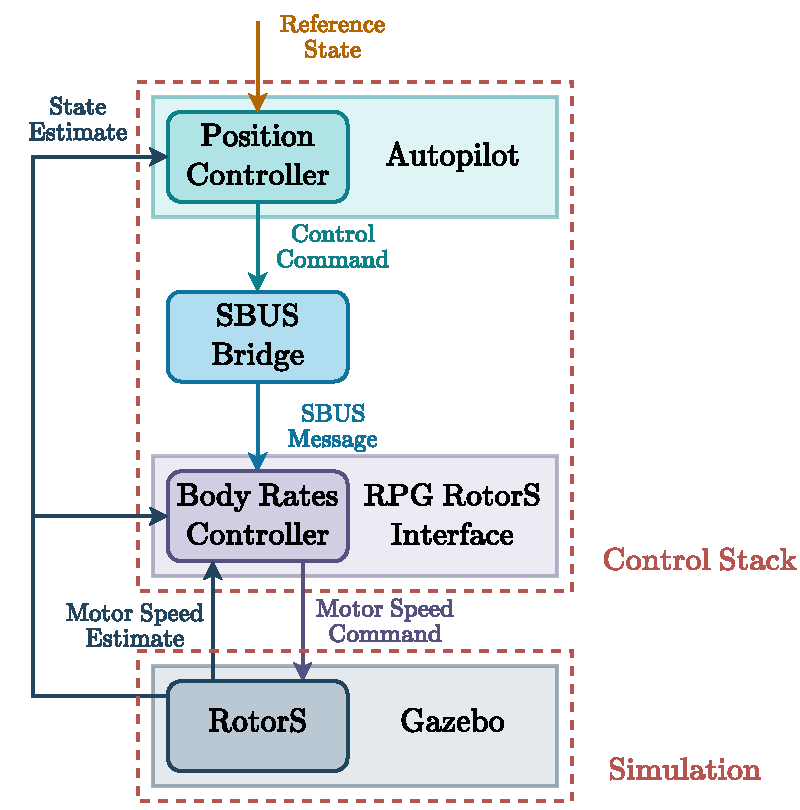
\includegraphics[width=0.7\textwidth]{own/control_module.drawio.pdf}
    \caption[
        The control stack in simulation.
    ]{
        The control stack in simulation.
        \label{fig:control_module}}
\end{figure}

The RPG Quadrotor Control implementation,
which includes the autopilot, the SBUS bridge and and the RPG RotorS interface,
basically executes two feedback control loops in a cascade.
The autopilot integrates the position controller 
that runs the control algorithm of Faessler at al. proposed in \cite{Faessler2018}.
Based on the latest reference state and the fed back drone state estimates,
the position controller generates high-level control commands.
A control command comprises 
the collective thrust of the drone's rotors 
as well as the drone's angular velocity and acceleration.
The SBUS bridge converts each incoming control command
into an SBUS message and forwards this message to the
RPG RotorS interface.
The RPG RotorS interface integrates the body-rate controller
that runs the control algorithm of Faessler at al. proposed in \cite{Faessler2017}.
Based on the latest high-level control command 
as well as the fed back drone state and motor speed estimates,
the body-rate controller generates low-level motor speed commands.
These commands are forwarded to RotorS for execution.
RotorS, developed by Furrer et al. \cite{Furrer2016},
is plugged into the Gazebo \footnote{
    \url{https://gazebosim.org/home}, visited on 18/08/2022
}
simulator to model the drone's physics 
and to provide the controllers with
drone state and motor speed estimates.

In real-world, the drone's flight controller would replace the 
RPG RotorS interface in order to generate hardware-specific low-level
motor commands based on the latest SBUS message from the SBUS bridge.








\section{Expert system} \label{sec:expert_system}
%In contrast to the ANN module,
%the expert system derives its navigation decisions 
%not from onboard sensor data but from its knowledge base.
%The task of the ANN module 
%is to infer navigation decisions,
%i.e., the inputs of the planning module,
%from onboard sensor data.
%In order to make meaningful decisions
%that successfully guide the drone through the racetrack,
%the ANN module must be previously trained on training data 
%of sufficient quantity and quality.
%To guarantee both,
%the training data is automatically generated 
%while the drone is flying through the racetrack.
%At training data generation (see XXX),
%the expert system undertakes the task
%of the completely untrained or yet insufficiently trained ANN module
%to make navigation decisions.

In the context of machine learning, 
an expert system is a program that imitates a human expert
in order to solve a problem. 
It comprises a knowledge base,
which stores known facts and rules, and an
inference engine, which infers new facts 
by applying the rules to the known facts \cite{osti_5675197}.

\paragraph*{Problem} $\ $\\
This thesis implements the expert system 
by Kaufmann et al. \cite{Kaufmann2018}
in order to solve the problem of automated navigation decision making
during the generation of training data for the ANN module.
The training dataset is extended with new samples 
while the drone runs the autonomous navigation method to fly through a racetrack.
The expert system checks the latest navigation decision 
made by the yet partially trained ANN module.
If it does not meet certain requirements,
the expert system intervenes with its own navigation decision.
This, first, keeps the drone on course and, second,
triggers the generation of a new training sample labeled 
with the expert system's navigation decision.

\paragraph*{Knowledge base} $\ $\\
While the ANN module infers navigation decisions from onboard sensor data,
the expert system makes navigation decisions based on its knowledge
which includes the following known facts (\textbf{F*}) and rules (\textbf{R*}).
\begin{itemize}
    
    \item [\textbf{F1}] 
    The planning module's waypoint
    \begin{equation}
        \pos[]{\text{ann}}{\wayp}{\grs}{}
    \end{equation}
     with respect to the global reference system
    (see equ. \ref{eq:pl_global_wayp}) 
    that was computed based
    on the ANN module's latest navigation decision
    (see equ. \ref{eq:navigation_decision}).
    

    \item [\textbf{F2}] The drone's latest position and quaternion orientation estimate,
    which are provided by the drone's state estimation system and 
    may correspond to ground truth in the simulation
    \begin{equation}
        \pos[]{\drone}{}{\grs}{}
        ,\quad 
        \quat[]{\drone}{}{\grs}{}.
    \end{equation}
    
    \item [\textbf{F3}] The center points of the gates of the racetrack
    \begin{equation}
        \left( 
            \pos[]{\gate}{\idx[]{}{}{}{}}{\grs}{}
        \right)
        _{\idx[]{}{}{}{} \in \left\{0, ..., \num[]{\gate}{}{}{} - 1 \right\}}
    \end{equation}
    and the initial index to the currently targeted gate to be passed next
    \begin{equation}
        \idx[]{\gate}{\target}{}{} \in \left\{0, ..., \num[]{\gate}{}{}{} - 1 \right\}
        .
    \end{equation}

    \item [\textbf{R1}] Compute the global trajectory of the current racetrack
    \begin{align} \label{eq:glo_traj}
        \pos[]{\glotraj}{}{\grs}{}
        :\ 
        &\left[
            \timepnt[]{\gate}{0}{}{}, 
            \timepnt[]{\gate}{\num[]{\gate}{}{}{}}{}{}
        \right] \rightarrow \mathbb{R}^3
        ;\quad
        \timepnt[]{}{}{}{}
        \mapsto
        \pos[]{\glotraj}{}{\grs}{}(\timepnt[]{}{}{}{})
        .
    \end{align}
    The algorithm of Mellinger and Kumar \cite{Mellinger2011}
    finds the minimum snap (fourth time derivative of position) spline trajectory
    \begin{align}
        \pos[]{\glotraj}{}{\grs}{}(\timepnt[]{}{}{}{})
        = \sum_{i = 0}^{\num[]{\gate}{}{}{} - 1}
        \begin{cases}
            \pos[]{\glotraj}{i}{\grs}{}(\timepnt[]{}{}{}{})
            , 
            &t \in \left[\timepnt[]{\gate}{i}{}{}, \timepnt[]{\gate}{i+1}{}{}\right] \\
            0, & \text{else}
        \end{cases}
    \end{align}
    that, traverses through all gate center points (\textbf{F3}),
    each at its corresponding gate time $\timepnt[]{\gate}{i}{}{}$,
    and reconnects to itself at $t=\timepnt[]{\gate}{\num[]{\gate}{}{}{}}{}{}$ at gate $i=0$.
    The entries of the pieces 
    $\pos[]{\glotraj}{i}{\grs}{}(\timepnt[]{}{}{}{})$
    of the spline are polynomials. 
    The user specifies the polynomial order 
    $\num[\user]{\glotraj}{\text{poly}}{}{}$
    of the pieces and
    the continuity order
    $\num[\user]{\glotraj}{\text{cont}}{}{}$
    of the spline. 
    However, since the goal is to minimize snap,
    it is required that 
    $
    \num[\user]{\glotraj}{\text{poly}}{}{}
    \ge \num[\user]{\glotraj}{\text{cont}}{}{} \ge 4
    $.
    The algorithm performs the following two-step iterative optimization.

    First,
    the optimal polynomial coefficients of the spline pieces
    are found for fixed gate arrival times 
    $\timepnt[]{\gate}{i}{}{}$
    by solving the optimization problem
    \begin{align}
        &\qquad \argmin{\pos[]{\glotraj}{}{\grs}{}}
        \int_{\timepnt[]{\gate}{0}{}{}}^{\timepnt[]{\gate}{\num[]{\gate}{}{}{}}{}{}}
            \left\|
                \pos[\ddddot]{\glotraj}{}{\grs}{}(\timepnt[]{}{}{}{})
            \right\|^2_2
        \text d \timepnt[]{}{}{}{}
        \nonumber 
        \\
        \text{s.t.}\quad
        & \pos[]{\glotraj}{}{\grs}{}\left(\timepnt[]{\gate}{i}{}{}\right) = 
            \pos[]{\gate}{\idx[]{}{}{}{}}{\grs}{},
        &&
            \frac{\text d^j \pos[]{\glotraj}{}{\grs}{}}{\text d \timepnt[]{j}{}{}{}} 
            (\timepnt[]{\gate}{i}{}{}) \text{ defined},
        \nonumber \\
        & \idx[]{}{}{}{} \in \left\{0, ..., \num[]{\gate}{}{}{}\right\},
        && j \in \left\{1, ..., \num[\user]{\glotraj}{\text{cont}}{}{}\right\}.
    \end{align}
    Note that, as the spline is closed, 
    the first and last gate equate 
    $\pos[]{\gate}{\num[]{\gate}{}{}{}}{\grs}{} = \pos[]{\gate}{0}{\grs}{}$.
    Morover, the gate times of the very first iteration are 
    approximated with the distances between the gate center points
    devided by the user-specified maximum speed $\speed[\user]{\glotraj}{\mxm}{}{}$ of the trajectory.
    The above optimization problem
    is temporally and spatially dedimensionalized 
    to increase numeric stability and 
    reformulated as quadratic program,
    which is solved with the Gurobi\footnote{
        \url{https://www.gurobi.com/}, visited on 20/08/2022
    } optimizer.

    Second, the polynomial coefficients of the spline pieces 
    are fixed
    and the inner gate times
    $\timepnt[]{\gate}{i}{}{}$
    are optimized relatively to each other.
    The corresponding optimization problem
    \begin{align}
        &\qquad \argmin{\timepnt[]{\gate}{i}{}{}}
        \int_{\timepnt[]{\gate}{0}{}{}}^{\timepnt[]{\gate}{\num[]{\gate}{}{}{}}{}{}}
            \left\|
                \pos[\ddddot]{\glotraj}{}{\grs}{}(\timepnt[]{}{}{}{})
            \right\|^2_2
        \text d \timepnt[]{}{}{}{}
        \nonumber \\
        \text{s.t.}\quad
        & \timepnt[]{\gate}{i}{}{} < \timepnt[]{\gate}{i+1}{}{},
        \qquad
        \timepnt[]{\gate}{0}{}{},\ \timepnt[]{\gate}{\num[]{\gate}{}{}{}}{}{} \text{ fixed},
        \qquad
        \idx[]{}{}{}{} \in \left\{0, ..., \num[]{\gate}{}{}{} - 1 \right\}
    \end{align}
    is solved by gradient descent with backtracking line search.

    
    
    The two optimization steps are executed iteratively until the cost
    of the first optimization problem converges. 
    Then, the trajectory is temporally and spatially redimensionalized
    and temporally scaled to adhere to 
    the user-specified maximum values in terms of 
    speed
    $\speed[\user]{\glotraj}{\mxm}{}{}$, 
    thrust 
    $\scacc[\user]{\glotraj}{\mxm}{}{}$
    and roll-pitch rate 
    $\scangvel[\user]{\glotraj}{\mxm}{}{}$
    along the trajectory. 
    For later use,
    the expert system samples the positions and speeds
    of the global trajectory
    \begin{equation}
        \left( 
            \pos[]{\glotraj}{\idx[]{}{}{}{}}{\grs}{}
        \right)
        _{\idx[]{}{}{}{} \in \left\{0, ..., \num[]{\glotraj}{}{}{} - 1 \right\}}
        ,\quad
        \left( 
            \speed[]{\glotraj}{\idx[]{}{}{}{}}{\grs}{}
        \right)
        _{\idx[]{}{}{}{} \in \left\{0, ..., \num[]{\glotraj}{}{}{} - 1 \right\}}
    \end{equation}
    with $\speed[]{\glotraj}{\idx[]{}{}{}{}}{\grs}{} = 
    \left\| 
        \pos[\dot]{\glotraj}{\idx[]{}{}{}{}}{\grs}{}
    \right\|_2 $.
    The sampling occurs at the
    user-specified frequency
    $\freq[\user]{\glotraj}{}{}{}$,
    which results in
    $\num[]{\glotraj}{}{}{} = \freq[\user]{\glotraj}{}{}{} \cdot 
    \left(\timepnt[]{\gate}{\num[]{\gate}{}{}{}}{}{}
    - \timepnt[]{\gate}{0}{}{}\right)$
    samples.

    
    \item [\textbf{R2}] If the drone is closer to the currently targeted gate 
    than a user-specified distance
    \begin{equation}
        \left\| 
            \pos[]{\gate}{\idx[]{\gate}{\target}{}{}}{\grs}{} - \pos[]{\drone}{}{\grs}{}
        \right\|_2 
        < 
        \dist[\user]{\dronetogate}{}{}{},
    \end{equation}
    increment the index to the currently targeted gate
    \begin{align}
        \idx[]{\gate}{}{}{} &\leftarrow (\idx[]{\gate}{}{}{} + 1) \bmod \num[]{\gate}{}{}{}.
    \end{align}
    
    \item [\textbf{R3}] If the
    planning module's waypoint (\textbf{F1}) computed based on the
    ANN module's latest navigation decision,
    is more distant from the global trajectory (\textbf{R1}) than
    a user-specified margin scaled by the 
    the user-specified drone's maximum speed, i.e.,
    \begin{equation}
        \argmin{i \in \{0, ..., \num[]{\glotraj}{}{}{} - 1\}}
            \left\| 
                \pos[]{\text{ann}}{\wayp}{\grs}{}
                - 
                \pos[]{\glotraj}{i}{\grs}{}
            \right\|_2
            >
            \dist[\user]{\wayptoglotraj}{\mxm}{}{} \cdot \frac{\speed[\user]{\drone}{\mxm}{}{} +1}{5},
    \end{equation}
    the expert system is required to intervene with its own navigation decision.

    
    \item [\textbf{R4}] Update the index 
    $\idx[]{\glotraj}{\proj}{}{} \in \{0, ..., \num[]{\glotraj}{}{}{} - 1\}$ 
    to the projection state,
    i.e., the state of the global trajectory
    onto which the drone's latest position estimate is projected,
    with the following iterative method.
    Figure \ref{fig:expert_system_projection} 
    schematically illustrates the method with a 2D example.
    \begin{enumerate}
        \item Compute the index to the previous state of the global trajectory,
        by decrementing the index to the projection state
        \begin{equation}
            \idx[]{\glotraj}{\prev}{}{} 
            = 
            (\idx[]{\glotraj}{\proj}{}{} - 1 + \num[]{\glotraj}{}{}{}) 
            \bmod 
            \num[]{\glotraj}{}{}{}.
        \end{equation}
        \item Starting from the previous state, 
        compute the vector to the projection state
        \begin{equation} \label{eq:vec_prev_state_2_proj_state}
            \anything[]{}{}{\grs}{}{\underline a}
            = 
            \pos[]{\glotraj}{\idx[]{\glotraj}{\proj}{}{}}{\grs}{}
            - 
            \pos[]{\glotraj}{\idx[]{\glotraj}{\prev}{}{}}{\grs}{}
        \end{equation}
        and the vector to the current drone position
        \begin{equation} \label{eq:vec_prev_state_2_drone}
            \anything[]{}{}{\grs}{}{\underline b}
            = 
            \pos[]{\drone}{}{\grs}{}
            - 
            \pos[]{\glotraj}{\idx[]{\glotraj}{\prev}{}{}}{\grs}{}.
        \end{equation}
        \item If the scalar product of the vectors 
        $\anything[]{}{}{\grs}{}{\underline a}$ 
        and 
        $\anything[]{}{}{\grs}{}{\underline b}$, 
        both normalized by the length of $\anything[]{}{}{\grs}{}{\underline a}$,
        is less than 1
        \begin{align} \label{eq:norm_dot_prod_criterion}
            \frac{
                \anything[]{}{}{\grs}{}{\underline a} 
                \cdot 
                \anything[]{}{}{\grs}{}{\underline b}
            }{  
                \anything[]{}{}{\grs}{}{\underline a} 
                \cdot 
                \anything[]{}{}{\grs}{}{\underline a}
            } < 1,
        \end{align}
        go to the next step. 
        Else, increment the index to the projection state
        \begin{equation}
            \idx[]{\glotraj}{\proj}{}{} 
            \leftarrow 
            (\idx[]{\glotraj}{\proj}{}{} + 1) \bmod \num[]{\glotraj}{}{}{}
        \end{equation}
        and go back to step 1.
        \item If the drone is 
        within a user-specified distance to the projection state 
        \begin{equation} \label{eq:dist_drone_proj_criterion}
            \left\| 
                \pos[]{\drone}{}{\grs}{}
                - 
                \pos[]{\glotraj}{\idx[]{\glotraj}{\proj}{}{}}{\grs}{}
            \right\|_2 
            \le 
            \dist[\user]{\dronetoproj}{}{}{},
        \end{equation}
        the index 
        $\idx[]{\glotraj}{\proj}{}{}$ 
        to the projection state is found.
        Else, set the index 
        to the state of the global trajectory
        which has the minimum distance to the current drone position
        \begin{equation} \label{eq:proj_idx_with_min_dist}
            \argmin{\idx[]{\glotraj}{\proj}{}{}}
            \left\| 
                \pos[]{\drone}{}{\grs}{}
                - 
                \pos[]{\glotraj}{\idx[]{\glotraj}{\proj}{}{}}{\grs}{}
            \right\|_2.
        \end{equation}
        Due to this step,
        the expert system does not require to know
        the initial index 
        to the projection state.

    \end{enumerate}
    
    

    \begin{figure}
        \centering
        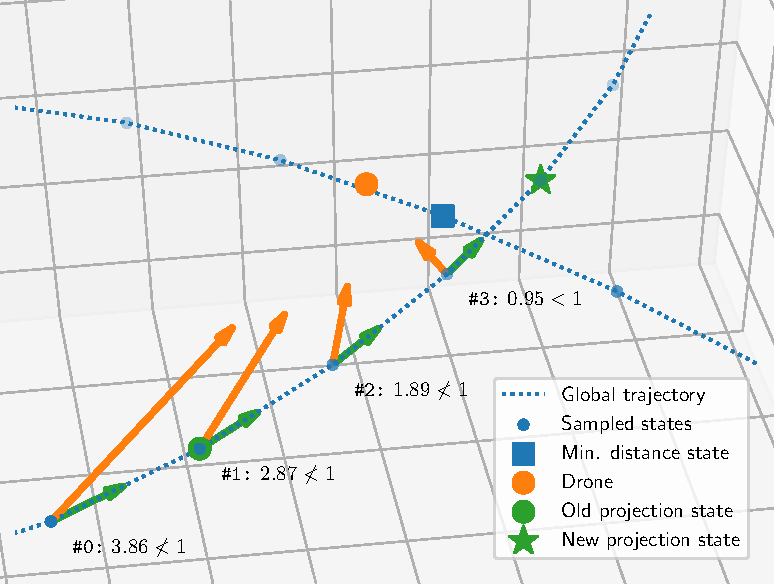
\includegraphics[width=0.9\textwidth]{own/expert_state_projection_3d.pdf}
        \caption[
            Update of the projection state index
        ]{
            Schematic example
            of the update of the projection state index (\textbf{R4}).
            Known are: the positions (blue points) 
            sampled from the global trajectory (blue dotted line),
            the last index to the projection state (green circle)
            and the current position of the drone (orange circle).
            At an iteration,
            the vector from the previous to the projection state 
            (green arrows, equ. \ref{eq:vec_prev_state_2_proj_state})
            and the vector from the previous to the drone position 
            (orange arrows, equ. \ref{eq:vec_prev_state_2_drone})
            are computed.
            Then, the normalized dot product criterion 
            (annotations, equ. \ref{eq:norm_dot_prod_criterion}) 
            is checked. 
            For iteration \#0-2, the criterion is not met.
            Thus, the index to the projection state is incremented
            and another iteration is started.
            At iteration \#3 the criterion is met and the 
            new index to the projection state (green star) is identified
            (assuming the distance criterion 
            (equ. \ref{eq:dist_drone_proj_criterion}) is also met). 
            Note that finding the index to the projection state 
            only with minimum distance 
            (equ. \ref{eq:proj_idx_with_min_dist}) 
            would have failed here,
            since the so indexed state (blue square) 
            belongs to a later or earlier part of the global trajectory 
            which only intersects the current part.
        \label{fig:expert_system_projection}}
    \end{figure}


    
    \item [\textbf{R5}] 
    Update the index 
    $\idx[]{\glotraj}{v}{}{} \in \{0, ..., \num[]{\glotraj}{}{}{} - 1\}$
    to the speed state,
    i.e., the state of the global trajectory
    that is the reference for the normalized speed
    $\speed[\norm]{\expert}{\desired}{}{}$ component
    of the expert system's navigation decision,
    by finding the first state of the global trajectory 
    that follows the projection state
    with a specific distance.
    \begin{enumerate}
        \item Initialize the searched index with the index to the projection state
        \begin{equation}
            \idx[]{\glotraj}{v}{}{} = \idx[]{\glotraj}{\proj}{}{}.
        \end{equation}

        \item Increment the searched index
        \begin{equation}
            \idx[]{\glotraj}{v}{}{} \leftarrow (\idx[]{\glotraj}{v}{}{} + 1) \bmod \num[]{\glotraj}{}{}{}.
        \end{equation}
        \item If the speed state is further 
        from the projection state than a user-specified distance
        \begin{equation}
            \left\| 
                \pos[]{\glotraj}{\idx[]{\glotraj}{v}{}{}}{\grs}{}
                - 
                \pos[]{\glotraj}{\idx[]{\glotraj}{\proj}{}{}}{\grs}{}
            \right\|_2
            > 
            \dist[\user]{\projtospeed}{}{}{}
            .
        \end{equation}
        the searched index is found.
        Else, go back to step 2.
    \end{enumerate}


    \item [\textbf{R6}] 
    Update the index 
    $\idx[]{\glotraj}{\wayp}{}{} \in \{0, ..., \num[]{\glotraj}{}{}{} - 1\}$
    to the waypoint state,
    i.e., the state of the global trajectory
    that is the reference for the image waypoint
    $\pos[]{\expert}{\wayp}{\irs}{}$
    component of the expert system's navigation decision,
    by finding the first state of the global trajectory 
    that follows the projection state
    with a distance to be computed.
    \begin{enumerate}
        \item Set the distance from the projection to the waypoint state
        to the distance from the drone to the closer of
        either the currently or lastly targeted gate.
        However, a user-specified distance constitutes the lower limit
        \begin{align}
            \dist[]{\projtowayp}{}{}{} &= 
            \maxof{
                \dist[\user]{\projtowayp}{\mnm}{}{}
            }{
                \argmin{i} \left\| 
                    \pos[]{\gate}{i}{\grs}{} 
                    - 
                    \pos[]{\drone}{}{\grs}{}
                \right\|_2
            }, 
            \\
            i &\in \left\{ \idx[]{\gate}{\target}{}{}, 
            (\idx[]{\gate}{\target}{}{} - 1 + \num[]{\gate}{}{}{}) 
            \bmod 
            \num[]{\gate}{}{}{}
            \right\}
            .
        \end{align}
        \item Initialize the searched index with the index to the projection state
        \begin{equation}
            \idx[]{\glotraj}{\wayp}{}{} = \idx[]{\glotraj}{\proj}{}{}.
        \end{equation}
        \item Increment the searched index
        \begin{equation}
            \idx[]{\glotraj}{\wayp}{}{} \leftarrow (\idx[]{\glotraj}{\wayp}{}{} + 1) 
            \bmod \num[]{\glotraj}{}{}{}.
        \end{equation}
        \item If the waypoint state is further from the projection state 
        than the distance computed in step 1
        \begin{equation}
            \left\| 
                \pos[]{\glotraj}{\idx[]{\glotraj}{\wayp}{}{}}{\grs}{}
                - 
                \pos[]{\glotraj}{\idx[]{\glotraj}{\proj}{}{}}{\grs}{}
            \right\|_2
            > 
            \dist[]{\projtowayp}{}{}{},
        \end{equation}
        the searched index is found.
        Else, go back to step 3.
    \end{enumerate}


    


    \item [\textbf{R7}] Compute the normalized speed component
    of the expert system's navigation decision
    as the sampled speed of the speed state
    normalized by the maximum speed of the global trajectory
    \begin{equation}
        \speed[\norm]{\expert}{\desired}{}{}
        = 
        \frac{
            \speed[]{\glotraj}{\idx[]{\glotraj}{v}{}{}}{\grs}{}
        }
        {
            \argmax{i \in \{0, ..., \num[]{\glotraj}{}{}{} - 1\}}
            \left\| 
                \speed[]{\glotraj}{\idx[]{}{}{}{}}{\grs}{}
            \right\|_2
        }  
        \in [0,1].
    \end{equation}


    
    
    
    \item [\textbf{R8}] Compute the image waypoint component
    of the expert system's navigation decision
    by applying the transformation
    from the global to the image reference system (see equ. \ref{eq:global_image_transformations})
    on the sampled position of the waypoint state 
    \begin{equation}
        \pos[]{\expert}{\wayp}{\irs}{}
        =
        \trafo[]{}{\irs\grs}{}{} \left(
            \pos[]{\glotraj}{\idx[]{\glotraj}{\wayp}{}{}}{\irs}{}
        \right)
        .
    \end{equation}

\end{itemize}





\paragraph*{Inference Engine} $\ $\\
The inference engine of the expert system is only activated 
during training data generation.
Figure ?? shows the related interaction of the inference engine 
within the autnomous navigation method.
Internally, the inference engine runs the following schedule.

Before the drone starts to fly,
the inference engine pre-computes the global trajectory (\textbf{R1})
and samples the position and speeds.
During the flight, it constantly update the currently targeted
gate index (\textbf{R2}).
Whenever the planning module has computed a global waypoint on the basis
of the latest ANN navigation decision,
the inference engine checks whether it must intervene (\textbf{R3}).
If so, the engine updates its indices to relevant states of the global trajectory
(\textbf{R4-6})
and makes its own navigation decision (\textbf{R7-8}).
Finally the engine sends its navigation decision to the planning module for processing.

\section{Racing vs. Training Data Generation}





